\section{Excercise CarRentalStructs}
\label{sec:car_rental_structs}

\subsection*{Add the Attributes to Structs}
After adding the attributes from the entity diagram to the 
\texttt{.../golang/CarRental/CarRentalStructs/CarRentalStructs.go} path and saving
the IDE automatically formats the code and indents it correctly.

\subsection*{Initialize and Print Structs}
The result of the initialization and printing of the structs is shown in figure \ref{fig:car_rental_structs}.
\begin{figure}[H]
    \centering
    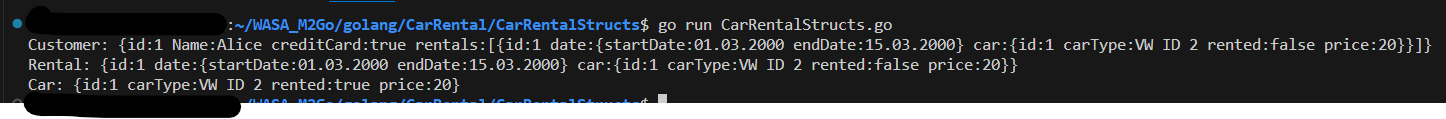
\includegraphics[width=\textwidth]{figures/goLang/carRental/carRental_structs.png}
    \caption{Output of the structs}
    \label{fig:car_rental_structs}
\end{figure}

\subsection*{Create an Array of Rentals}
The function works as follows:
\begin{enumerate}
    \item The array \texttt{cartypes} holds the string of 5 different cartypes
    \item The function \texttt{createRentals(id, date, car)} returns 5 rentals that are appended to the array
    \item Via \texttt{fmt.Println(rentals)} the array is printed into the console
\end{enumerate}

The result looks like this:
\begin{figure}
    \centering
    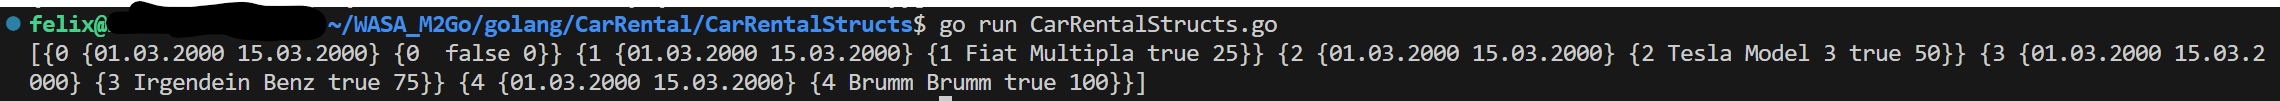
\includegraphics{figures/goLang/carRental/carRental_arrayFiveRentals.png}
    \caption{Output of the Array of Rentals}
    \label{fig:car_rental_array_five_rentals}
\end{figure}
